%input macros (i.e. write your own macros file called MacroFile1.tex)
%\include{Macros/MacroFile1}

\documentclass[oneside,12pt]{Classes/CUEDthesisPSnPDF}
\usepackage{epstopdf}

%
%    \pdfinfo { /Title  (MTech Dessertation)
%               /Creator (TeX)
%               /Producer (pdfTeX)
%               /Author (AmritaWNA)
%               /CreationDate (D:20110520)  %format D:YYYYMMDD
%               /ModDate (D:20110520)
%               /Subject (Writing a Dessertation in LaTeX)
%               /Keywords (MTech, Thesis)}
%    \pdfcatalog { /PageMode (/UseOutlines)
%                  /OpenAction (fitbh)  }
%               
                  
   % Change the Title as per your details
		\title{Node Failures and its Impact on Data Aggregation Delay} 
		\degree{MASTER of TECHNOLOGY \\[1ex]IN \\[1ex]WIRELESS NETWORKS AND APPLICATIONS}
		
		% The year and Month the degree will be officially conferred
		\degreedate{April 2013}      
		% Change the Author name to full name of the person submitting the report.                   
		\author{Sreedevi A. G.}
		% Change the Guide name to full name of the Guide.  
		\guide{Dr. P Venkat Rangan}
		% Change the register no.  
		\regno{AM.EN.P2WNA10018}
		% Change the Academic Year
		\academicyear{2012-2013}
	  \crest{
\includegraphics[width=60mm]{UniEmblem.eps}}
  	\collegeordept{AMRITA CENTER FOR WIRELESS NETWORKS AND APPLICATIONS}
	  \university{AMRITA VISHWA VIDYAPEETHAM (AMRITA UNIVERSITY),\\[1ex] (Estd. U/S 3 of the UGC Act 1956) Amritapuri  Campus \\[1ex] Kollam -690525}
  	\crestsmall{
\includegraphics[width=30mm]{UniEmblem.eps}}
% Packages that are used  
\usepackage{subfig,enumerate,algorithm,algorithmic,fancyvrb,amsthm}
\usepackage{multirow}

\begin{document}

\maketitle

\begin{center}
{\normalsize {\bfseries{AMRITA CENTER FOR WIRELESS NETWORKS AND APPLICATIONS	\\[1ex]}}}
{\normalsize {\bfseries{AMRITA VISHWA VIDYAPEETHAM (AMRITA UNIVERSITY),\\[1ex] (Estd. U/S 3 of the UGC Act 1956) Amritapuri  Campus \\[1ex] Kollam -690525\\[1ex]}}}
	
\includegraphics[width=30mm]{UniEmblem.eps}
	\\[1ex]					
				\rmfamily\bfseries\upshape\Large
				BONAFIDE CERTIFICATE \\[2ex] % Insert your Project title here
\end{center}
		\vspace{1pt}	
\rmfamily\mdseries\upshape\normalsize					
%\begin{flushleft}
This is to certify that the Seminar Report entitled \textbf{``Node Failures and its Impact on Data Aggregation Delay in Hierarchical WSNs''} submitted by \textbf{Ms. Sreedevi A. G.(AM.EN.P2WNA10018)}, in partial fulfillment of the degree of Master of Technology in Amrita Center for Wireless Networks and Applications, Amrita Vishwa Vidyapeetham (Amrita University), is a bonafide record of the work carried out by him/her  at Amrita School of Engineering, Amritapuri during Semester 2 of the academic year 2012-2013. 
%\end{flushleft}
			
\vspace{45pt}
\begin{flushleft}
Coordinator\hspace{200pt} Head of the Department\\
\vspace{3pt}
Prof. K A Unnikrishna Menon\hspace{100pt} Dr. Maneesha V Ramesh\\
\vspace{40pt}
\end{flushleft}
\begin{flushleft}
\vspace{5pt}
Place	:	Amritapuri \\
Date	:	56 July, 2056
\end{flushleft}


\pagebreak

\begin{center}
   {\normalsize {\bfseries{AMRITA CENTER FOR WIRELESS NETWORKS AND APPLICATIONS	\\[1ex]}}}

    {\normalsize {\bfseries{AMRITA VISHWA VIDYAPEETHAM (AMRITA UNIVERSITY),\\[1ex] (Estd. U/S 3 of the UGC Act 1956) Amritapuri  Campus \\[1ex] Kollam -690525\\[1ex]}}}
    
\includegraphics[width=30mm]{UniEmblem.eps}
	\\[1ex]	
    \rmfamily\bfseries\upshape\Large
				DECLARATION \\[2ex]
    %
\includegraphics[width=30mm]{UniEmblem}
    
    \end{center}
	\vspace{2pt}
I, \textbf{Ms. Sreedevi A. G., Reg No:AM.EN.P2WNA10018}, hereby declare that this seminar entitled 
\textbf{"Node Failures and its Impact on Data Aggregation Delay in Hierarchical WSNs"} is a record of the literature work done at Amrita Center for Wireless Networks and Applications, Amrita Vishwa Vidyapeetham (AMRITA UNIVERSITY), that this work has not formed the basis for any degree/diploma/associationship/fellowship or similar awards to any candidate in any university to the best of my knowledge.

\vspace{60pt}
\begin{flushleft}
Place	:	Amritapuri% PRint the place and date
\\[1ex]
Date	:	67th July, 2096.
\\[15ex]
Signature of the Student 
\end{flushleft}

%set the number of sectioning levels that get number and appear in the contents
\setcounter{secnumdepth}{3}
\setcounter{tocdepth}{3}

\frontmatter % book mode only
\pagenumbering{roman}
\include{Dedication/dedication}
% Thesis Acknowledgements ------------------------------------------------


%\begin{acknowledgementslong} %uncommenting this line, gives a different acknowledgements heading
\begin{acknowledgements}      %this creates the heading for the acknowlegments

The acknowledgement listed below is just a sample for you to understand. Write appropriate acknowledgement w.r.t you seminar work. It is recomented not to use the same sentences listed below!...
I would like to thank my advisor, Dr. P Venkat Rangan for his tireless mentorship and support. I would also like to express my sincere gratitude to Prof. Unnikrishna Menon and Mr. Arun Balakrishann, the seminar coordinators  for their immense support and the time they dedicated to help me solving my doubts at various stages of the research.\\[1ex]
Thapasya\\
I am also indebted to Professors Maneesha V Ramesh,  and Balaji Hariharan for their research collaboration and their excellent teaching. I would also thank all faculty members of Amrita Center for Wireless Networks and Applications for their co-operation in completing this seminar. I also thank to my colleagues for the time they dedicated to discuss various research problems with me and for the spirit of camaraderie they helped foster in our laboratory.\\[1ex]

I would also like to express my gratitude for the immeasurable motivation and guidance provided by Sri. Mata Amritanandamayi Devi (AMMA), Chancellor of Amrita University. Above all, I thank God Almighty for his grace, for giving me strength and ideas for making this seminar work, flow smoothly.\\[1ex]

\end{acknowledgements}
%\end{acknowledgmentslong}

% ------------------------------------------------------------------------

%%% Local Variables: 
%%% mode: latex
%%% TeX-master: "../thesis"
%%% End: 


% Thesis Abstract -----------------------------------------------------


%\begin{abstractslong}    %uncommenting this line, gives a different abstract heading
\begin{abstracts}        %this creates the heading for the abstract page

You can write your seminar work abstract in short here. 

\end{abstracts}
%\end{abstractlongs}


% ----------------------------------------------------------------------


%%% Local Variables: 
%%% mode: latex
%%% TeX-master: "../thesis"
%%% End: 


\tableofcontents
\listoffigures
\listoftables
\listofalgorithms
\printnomenclature  %% Print the nomenclature
\addcontentsline{toc}{chapter}{Nomenclature}

\mainmatter % book mode only
%%% Thesis Introduction --------------------------------------------------
\chapter{Introduction}


\ifpdf
    \graphicspath{{Introduction/IntroductionFigs/PNG/}{Introduction/IntroductionFigs/PDF/}{Introduction/IntroductionFigs/}}
\else
  \graphicspath{{Introduction/IntroductionFigs/EPS/}{Introduction/IntroductionFigs/}}
\fi

\section{Overview}
\markboth{}{Node Failures and its Impact on Data Aggregation Delay}{}

This chapter can explain the introduction in general to your seminar work. then specifically you can have sub sections and sub-sub sections to explain each and every sub-area of your work. It can include a general introduction, advantages and challenges of the area.\\[1ex]

The rest of the report is organized as follows: A literature survey is presented in section 2. Two level Balanced and Progressive sensor network topologies and their energy optimization are described in section 3. In sections 4 to 6, we analyse node failure handling strategies in different levels of the Balanced and Progressive two level tree WSNs and propose solutions. Section 7 contains results and observations. Finally we conclude in section 8. \\[1ex]

\section{New Section}
%\markboth{}{\MakeUppercase{\thechapter.  Introduction }}
contents for section here....
\subsection{Subsection1}
You can write contents for your subsection here...

\subsection{Subsection2}

You can write contents for your subsection here...


\section{Another Section}
\markboth{}{Node Failures and its Impact on Data Aggregation Delay}{}

%\markboth{\MakeUppercase{\thechapter. Introduction }}

The enumeration:\\[1ex]
\begin{enumerate}
\item \textbf{Enum1}: Explanation1
\item \textbf{Enum2}: Explanation2
\end{enumerate}

The figure \ref{fig1} is \cite{RW1} : \\[1ex]

\begin{figure}[t]
\centering
\subfloat[Without In-Network Data Aggregation]{\includegraphics[width = 2.5in]{fig1.eps}}
\qquad
\subfloat[With In-Network Data Aggregation]{\includegraphics[width = 2.5in]{fig2.eps}}
\caption{In-Network Data Aggregation}
\label{fig1}
\end{figure}

Itemization: \\[1ex]
\begin{itemize}
\item Centralized Approach: This is an address centric approach where each node sends data to a central node via the shortest possible route using a multi hop wireless protocol.
\item In-Network Aggregation: In-network aggregation is the global process of gathering and routing information through a multi-hop network, processing data at intermediate nodes with the objective of reducing resource consumption (in particular energy), thereby increasing network lifetime. 
\item Tree-Based Approach: In the tree-based approach perform aggregation by constructing an aggregation tree, which could be a minimum spanning tree, rooted at sink and source nodes are considered as leaves.
\item Cluster-Based Approach: In cluster-based approach, whole network is divided in to several clusters. Each cluster has a cluster-head which is selected among cluster members \cite{RW2}.
\end{itemize}


%% Local Variables: 
%%% mode: latex
%%% TeX-master: "../thesis"
%%% End: 

% \pagebreak[4]
% \hspace*{1cm}
% \pagebreak[4]
% \hspace*{1cm}
% \pagebreak[4]

\chapter{Related Works}
%\markboth{}{\MakeUppercase{\thechapter. Related Works }}
\markboth{}{Node Failures and its Impact on Data Aggregation Delay}{}

This section should explain the literature survey of your work. You can have sections and subsections explaining drawbacks of the current system or technology \cite{RW2}.\\[1ex]

\section{Drawbacks of the Current System}
\markboth{}{Node Failures and its Impact on Data Aggregation Delay}{}

This section should explain the literature survey of your work. You can have sections and subsections explaining drawbacks of the current system or technology \cite{RW2}.\\[1ex]



% ------------------------------------------------------------------------


%%% Local Variables: 
%%% mode: latex
%%% TeX-master: "../thesis"
%%% End: 

\chapter{Proposed System Titles}
\ifpdf
    \graphicspath{{Chapter2/Chapter2Figs/PNG/}{Chapter2/Chapter2Figs/PDF/}{Chapter2/Chapter2Figs/}}
\else
    \graphicspath{{Chapter2/Chapter2Figs/EPS/}{Chapter2/Chapter2Figs/}}
\fi

\section{Proposed System Title}
%\markboth{}{\MakeUppercase{\thechapter. Proposed System Title }}
\markboth{}{Node Failures and its Impact on Data Aggregation Delay}{}

\subsection{Subsection1}
You can write contents for your subsection here...

\subsection{Subsection2}

You can write contents for your subsection here...

\begin{table}[ht]
\caption{The Symbols Used in the Paper} % title of Table
\centering % used for centering table
\begin{tabular}{l p{9cm}} % centered columns (4 columns)
\hline\hline %inserts double horizontal lines
Symbol & Description \\ [0.5ex] % inserts table
%heading
\hline % inserts single horizontal line
$N$ & Amount of SNs in tree WSN \\ % inserting body of the table
$m$ & Amount of INs in tre WSN \\
$T_{comp}$ & Time taken for comparing two sensed values \\
$T_{net}$ & Transmission time from one wireless node to another in the WSN \\
\hline %inserts single line
\end{tabular}
\label{table:table1} % is used to refer this table in the text
\end{table}

The total energy consumed by the GN is proportional to the amount of computations and amount of transmissions. The total delay or energy consumed or time taken by the GN to complete the aggregate computation in a balanced two level tree WSN is,

\begin{equation}
T_{max} = {\frac{N}{m}-1}
\end{equation}

\begin{figure}[t] %inserts the figure at the top of the page t denotes the top of the page %[!htbp]
  \begin{center}
    \leavevmode  
      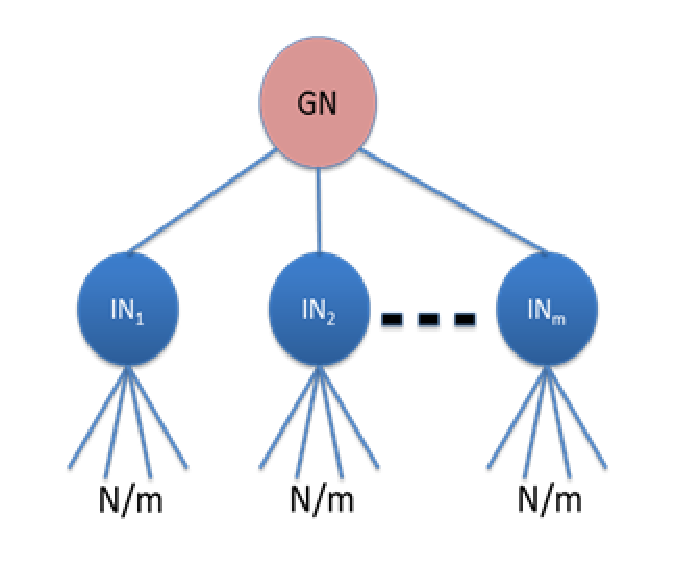
\includegraphics[height=2in]{5.eps}
     \caption{Balanced Two Level Tree WSN}     
    \label{bal}
  \end{center}
\end{figure}

% ------------------------------------------------------------------------

%%% Local Variables: 
%%% mode: latex
%%% TeX-master: "../thesis"
%%% End: 

\chapter{Advantages and Disadvantages of the System}
\ifpdf
    \graphicspath{{Chapter3/Chapter3Figs/PNG/}{Chapter3/Chapter3Figs/PDF/}{Chapter3/Chapter3Figs/}}
\else
    \graphicspath{{Chapter3/Chapter3Figs/EPS/}{Chapter3/Chapter3Figs/}}
\fi

\markboth{}{Node Failures and its Impact on Data Aggregation Delay}{}

\section{Advantages}
\markboth{}{Node Failures and its Impact on Data Aggregation Delay}{}

\section{Disadvantages}
\markboth{}{Node Failures and its Impact on Data Aggregation Delay}{}
%%% Local Variables: 
%%% mode: latex
%%% TeX-master: "../thesis"
%%% End: 

\chapter{Applicablity of the System in Other Areas}
\ifpdf
    \graphicspath{{Chapter4/Chapter4Figs/PNG/}{Chapter4/Chapter4Figs/PDF/}{Chapter4/Chapter4Figs/}}
\else
    \graphicspath{{Chapter4/Chapter4Figs/EPS/}{Chapter4/Chapter4Figs/}}
\fi

\markboth{}{Node Failures and its Impact on Data Aggregation Delay}{}



% ------------------------------------------------------------------------

%%% Local Variables: 
%%% mode: latex
%%% TeX-master: "../thesis"
%%% End: 

\def\baselinestretch{1}
\chapter{Conclusion}
\ifpdf
    \graphicspath{{Conclusions/ConclusionsFigs/PNG/}{Conclusions/ConclusionsFigs/PDF/}{Conclusions/ConclusionsFigs/}}
\else
    \graphicspath{{Conclusions/ConclusionsFigs/EPS/}{Conclusions/ConclusionsFigs/}}
\fi

\def\baselinestretch{1.66}
\markboth{}{Node Failures and its Impact on Data Aggregation Delay}{}



%%% ----------------------------------------------------------------------

% ------------------------------------------------------------------------

%%% Local Variables: 
%%% mode: latex
%%% TeX-master: "../thesis"
%%% End: 

\chapter{Future Work}
\ifpdf
    \graphicspath{{Chapter5/Chapter5Figs/PNG/}{Chapter5/Chapter5Figs/PDF/}{Chapter5/Chapter5Figs/}}
\else
    \graphicspath{{Chapter5/Chapter5Figs/EPS/}{Chapter5/Chapter5Figs/}}
\fi

\markboth{}{Node Failures and its Impact on Data Aggregation Delay}{}


% ------------------------------------------------------------------------

%%% Local Variables: 
%%% mode: latex
%%% TeX-master: "../thesis"
%%% End: 



\backmatter % book mode only
\appendix
\chapter{Appendix A}
\section{Section Name}
\subsection{Subsection Name}

\subsection{Pin Diagram}


%\begin{eqnarray}
%\end{eqnarray}
% ------------------------------------------------------------------------

%%% Local Variables: 
%%% mode: latex
%%% TeX-master: "../thesis"
%%% End: 

%\include{Appendix2/appendix2}
\bibliographystyle{IEEEtran}
%\bibliographystyle{Classes/CUEDbiblio}
%\bibliographystyle{Classes/ieeetr}
%\bibliographystyle{Classes/jmb} % bibliography style
\renewcommand{\bibname}{References}% changes default name Bibliography to References 

\bibliography{References/references} % References file

\end{document}
